%!TEX program = xelatex

\documentclass[compress]{beamer}
%--------------------------------------------------------------------------
% Common packages
%--------------------------------------------------------------------------

\definecolor{links}{HTML}{663000}
\hypersetup{colorlinks,linkcolor=,urlcolor=links}

\usepackage[english]{babel}
\usepackage{pgfpages} % required for notes on second screen
\usepackage{graphicx}

\usepackage{multicol}


\usepackage{tabularx,ragged2e}
\usepackage{booktabs}

\setlength{\emergencystretch}{3em}  % prevent overfull lines
\providecommand{\tightlist}{%
  \setlength{\itemsep}{0pt}\setlength{\parskip}{0pt}}


\usetheme{hri}

\usepackage{remreset}% tiny package containing just the \@removefromreset command
\makeatletter
\@removefromreset{subsection}{section}
\makeatother
\setcounter{subsection}{1}

\newcommand{\source}[2]{{\tiny\it Source: \href{#1}{#2}}}
\newcommand{\stmt}[1]{{\footnotesize \tt  #1}}

\usepackage{tikz}
\usetikzlibrary{mindmap,backgrounds,positioning,calc,matrix}

\graphicspath{{figs/part7/}}

\title{ROCO318 \newline Mobile and Humanoid Robots}
\subtitle{Part 7 -- Robot Control}
\date{}
\author{Séverin Lemaignan}
\institute{Centre for Neural Systems and Robotics\\{\bf Plymouth University}}

\begin{document}

\licenseframe{github.com/severin-lemaignan/module-mobile-and-humanoid-robots}

\maketitle

\begin{frame}[plain]{}

    \Large

    \centering
    How hard might it be?

\end{frame}


\begin{frame}{Let's thinker a little...}

    Let's imagine you want to build a robot that {\bf fetches beers from the fridge}
    and bring them back to you whenever you ask. It should {\bf not kill the cat},
    and it should {\bf politely greet your mum} whenever it sees her.

    \begin{columns}
        \begin{column}{0.5\linewidth}

            You have:
            \begin{itemize}
                \item a map with the important landmarks like {\tt fridge}
                \item the following modules:
            \end{itemize}
        \end{column}
        \begin{column}{0.5\linewidth}
            \begin{center}
                \resizebox{\linewidth}{!}{
                    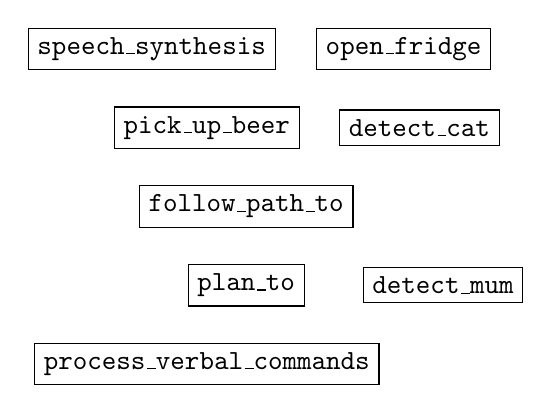
\begin{tikzpicture}[>=latex,every node/.style={draw,font=\tt}]

                        \node at (0.5,2) {follow\_path\_to};
                        \node at (2.5,4) {open\_fridge};
                        \node at (-0.7,4) {speech\_synthesis};
                        \node at (0,0) {process\_verbal\_commands};
                        \node at (3,1) {detect\_mum};
                        \node at (2.7,3) {detect\_cat};
                        \node at (0.5,1) {plan\_to};
                        \node at (0,3) {pick\_up\_beer};
                    \end{tikzpicture}
                }
            \end{center}
        \end{column}
    \end{columns}

    Can you draw a control architecture that achieves just that?
\end{frame}


\section{Control paradigms}

\begin{frame}{Behavioural (or reactive) control}

    {\bf Behaviours} are small programs that read sensors and control
    actuators. Each behaviour does \textbf{one simple thing}; it typically has
    access to all sensors/actuators.



    \begin{center}
        \only<1>{
        \resizebox{0.5\linewidth}{!}{
            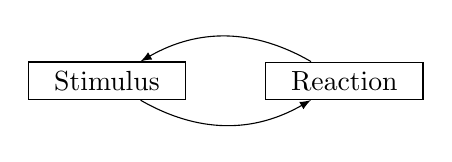
\begin{tikzpicture}[>=latex]
                \node[draw, minimum width=2cm,align=center] at (0,0) (stim) {Stimulus};
                \node[draw, minimum width=2cm,align=center,right=of stim] (reac) {Reaction};
                \path (stim) edge[bend right,->] (reac);
                \path (reac) edge[bend right,->] (stim);
            \end{tikzpicture}
            }
        }
        \only<2>{
        \resizebox{\linewidth}{!}{
            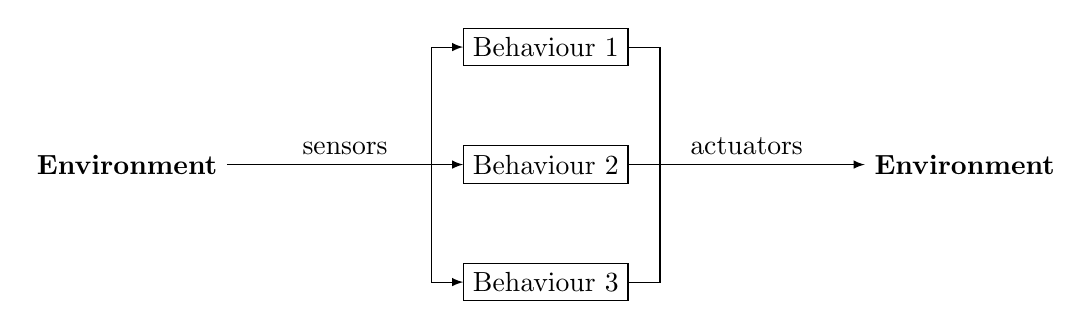
\begin{tikzpicture}[>=latex]
                \node[minimum width=2cm,align=center] at (0,0) (env) {\bf Environment};
                \node[draw, minimum width=2cm,align=center,right=3 of env] (b1) {Behaviour 2};
                \node[draw, minimum width=2cm,align=center,above=of b1] (b2) {Behaviour 1};
                \node[draw, minimum width=2cm,align=center,below=of b1] (b3) {Behaviour 3};
                \node[minimum width=2cm,align=center, right=3 of b1] (env2) {\bf Environment};
                \coordinate[left=0.4 of b1] (a);
                \coordinate[right=0.4 of b1] (b);

                \draw[->] (env)--node[anchor=south, midway]{sensors}(b1);
                \draw[->] (b1)--node[anchor=south, midway]{actuators}(env2);
                \draw[->] (a) |- (b2);
                \draw[->] (a) |- (b3);
                \draw (b) |- (b2);
                \draw (b) |- (b3);
            \end{tikzpicture}
            }

            We only want one behaviour at a time! Need to \textbf{prioritise}:
            behaviours can \emph{override} or \textbf{subsume} less important
            ones.

        }
    \end{center}
    
\end{frame}

\begin{frame}{Extreme case: Braitenberg machines}

    \begin{columns}
        \begin{column}{0.5\linewidth}

            \begin{itemize}
                \item Motion directly controlled by sensors (typically photocells)
                \item Yet the resulting behaviour may appear complex or even intelligent
                \item<1-2> Can you guess the behaviours of vehicles 2a and 2b?
                \item<3-> Complex behaviours emerge (typically with non-linear control functions).
            \end{itemize}

        \end{column}
        \begin{column}{0.5\linewidth}
            \begin{center}
                \includegraphics<1>[width=0.7\linewidth]{Braitenberg_Vehicle_2ab-blind}
                \includegraphics<2->[width=0.7\linewidth]{Braitenberg_Vehicle_2ab}

                \onslide<3>{
                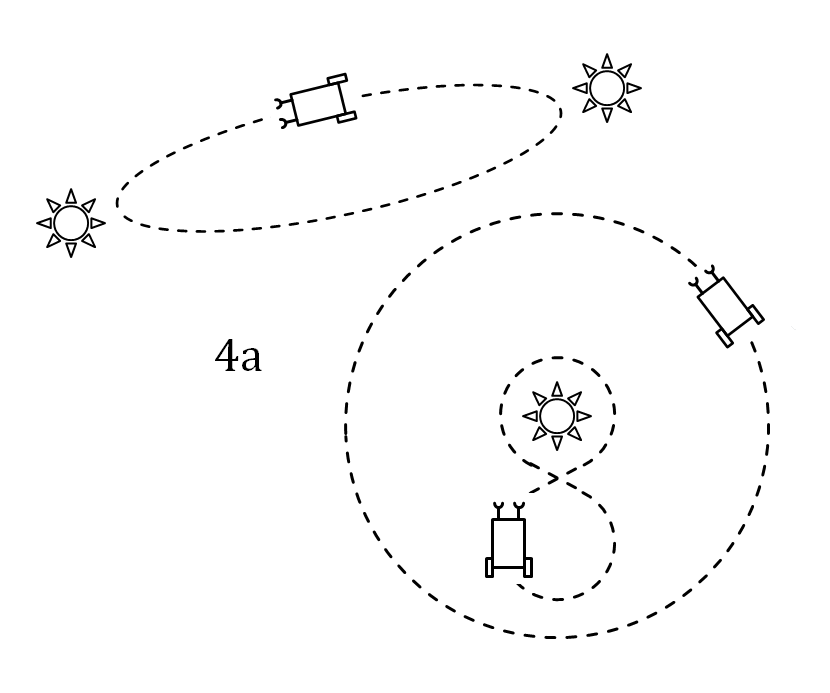
\includegraphics[width=0.7\linewidth]{Braitenberg_Vehicle_4a}
                }

                \source{https://en.wikipedia.org/wiki/Braitenberg_vehicle}{Wikipedia}
            \end{center}
        \end{column}
    \end{columns}

\end{frame}

\begin{frame}{Combining behaviours: example}

    \only<1>{

        Three behaviours:

        \begin{itemize}
            \item {\bf Follow a robot}
                \begin{itemize}
                    \item Sensor: IR communication
                    \item Behaviour: follow another robot
                \end{itemize}
            \item {\bf Avoid obstacle}
                \begin{itemize}
                    \item Sensors: bumpers
                    \item Behaviour: move away from the wall
                \end{itemize}
            \item {\bf Wander}
                \begin{itemize}
                    \item Sensors: encoders
                    \item Behaviour: move forward and turn
                \end{itemize}
        \end{itemize}

        Which behaviour should have the highest priority? the lowest?

        \source{https://www.clear.rice.edu/engi128/Handouts/Lec17-Robotics.pdf}{example borrowed from Rice University ENGI128}
    }
    \only<2->{
        \begin{center}
            \resizebox{0.6\linewidth}{!}{
                \begin{tikzpicture}[>=latex,
                                    every node/.style={draw,minimum width=2cm}]
                    \node at (0,0) (fol) {Follow a robot};
                    \node[below=1 of fol] (wander) {Wander};
                    \node[above=1 of fol] (avoid) {Avoid obstacle};

                    \node[left=1 of fol,anchor=center,rotate=90,minimum width=4cm] (sensors) {Sensors};

                    \draw[thick,->] (sensors) -- (fol);
                    \draw[thick,->] (sensors.south |- wander) -- (wander);
                    \draw[thick,->] (sensors.south |- avoid) -- (avoid);

                    \coordinate[right=1 of fol] (s1);
                    \coordinate[right=2 of wander] (s2);
                    \node[circle,ultra thick,fill=hriSec2Dark,minimum size=5mm] at (s1) (ss1) {\bf S};
                    \node[circle,ultra thick,fill=hriSec2Dark,minimum size=5mm] at (s2) (ss2) {\bf S};

                    \draw[<-] (ss1) -- ($(ss1) + (70:2cm)$) node[draw=none,align=center,above,color=hriSec1Dark] {\small\it subsumption\\ \small\it operator};

                    \draw[thick] (fol) -- (ss1);
                    \draw[thick,->] (avoid) -| (ss1);
                    \draw[thick] (wander) -- (ss2);
                    \draw[thick,->] (ss1) -| (ss2);

                    \node[right=3 of fol,anchor=center,rotate=-90,minimum width=4cm] (act) {Actuators};

                    \draw[thick,->] (ss2) -- (act.south |- ss2);

                    \node[draw=none, above=0.5 of avoid] {\small\emph{highest priority}};
                    \node[draw=none, below=0.5 of wander] {\small\emph{lowest priority}};

                \end{tikzpicture}
            }
        \end{center}

        We combine behaviours by {\bf subsuming} lower-priority behaviours
        whenever a higher-priority behaviour becomes active.

        \onslide<3>{
            $\rightarrow$ \textbf{subsumption architecture}
        }

    }

\end{frame}

\begin{frame}{Behavioural control: strengths/weaknesses}

    {\bf Strengths}

    \begin{itemize}
        \item {\bf Incremental development}
        \item By definition {\bf modular}
        \item Effective to react to events $\rightarrow$ well suited to {\bf
            dynamic environments}
    \end{itemize}

    {\bf Weaknesses}

    \begin{itemize}
        \item {\bf goal-oriented behaviours hard to implement} (``what will my robot do?'')
        \item {\bf importance of the arbiter}: who inhibits (\ie \emph{subsumes}) who might be context-dependent
        \item debugging difficult (need to trace which behaviours are active)
    \end{itemize}


\end{frame}

\begin{frame}{Event-oriented programming: example of Ranger}

    Ranger is a `box on wheels' developed at EPFL

    \begin{center}
        \includegraphics[width=\linewidth]{ranger}
    \end{center}
\end{frame}

\imageframe[color=black]{ranger-side}

\begin{frame}[fragile]{Event-oriented programming}

    {\bf Event-oriented programming} is a possible way of implementing a
    behavioural control paradigm:
    \vspace{1em}

\begin{overprint}
    \onslide<1>
\begin{pythoncode*}{frame=none}

with Ranger() as robot:

    robot.background_blink()
    robot.look_at_touches()

    robot.whenever("dummy", becomes = True)
                                .do(on_dummy)
    robot.whenever("dummy", becomes = False)
                                .do(on_dummy_removed)
    robot.whenever("scale", increase = 0.3).do(on_toy)
    robot.whenever("bumper", becomes = True).do(on_bumper)

    while True:
        time.sleep(0.1)
\end{pythoncode*}

    
    
    \onslide<2>
    \begin{columns}
        \begin{column}{0.45\linewidth}
            \begin{pythoncode*}{frame=none}
def on_dummy(robot):
    robot.look_at_dummy()
    robot.blink()
    sleep = robot.fall_asleep()
    robot.lightbar(RAINBOW).wait()
    sleep.wait()

def on_dummy_removed(robot):
    robot.light_bar(colors.rand())
    robot.wakeup().wait()
    robot.move(0.4, v = 0.8).wait()
    robot.idle().wait()

\end{pythoncode*}
\end{column}
        \begin{column}{0.55\linewidth}
\begin{pythoncode*}{frame=none}
def on_bumper(robot):
    pulse = robot.pulse_row(0)
    while abs(robot.state.v) > 0.01:
        robot.sleep(0.2)
    pulse.cancel()

def on_toy(robot):
    robot.playsound(SOUNDS["toy_in"])
    robot.lightbar(RAINBOW).wait()
\end{pythoncode*}
        \end{column}
    \end{columns}
\end{overprint}
\end{frame}

\imageframe[scale=0.8]{croquignole-expe}

\begin{frame}{}

    \begin{center}
        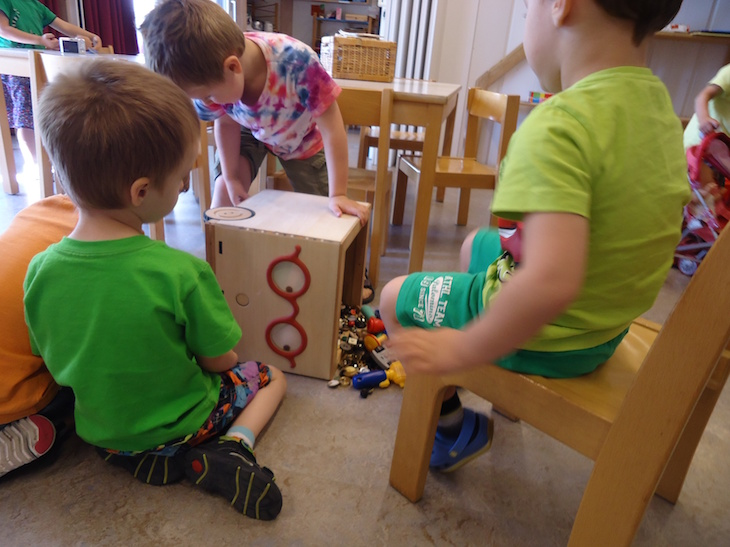
\includegraphics[width=0.7\linewidth]{ranger-side}

        Note that this is a example of {\bf aimless, purely reactive}, behaviour.
    \end{center}

\end{frame}

%%%%%%%%%%%%%%%%%%%%%%%%%%%%%%%%%%%%%%%%%%%%%%%%%%%%

\begin{frame}{Model-Plan-Act}

    Basic paradigm for {\bf deliberative architectures}.

    \begin{center}
        \resizebox{\linewidth}{!}{
            \begin{tikzpicture}[>=latex,
                                every node/.style={minimum width=4cm}]

                \node[minimum width=2cm] at (0,0) (env) {\bf Environment};
                \coordinate[right=3 of env] (c1);
                \coordinate[right=of c1] (c2);
                \coordinate[right=of c2] (c3);
                \coordinate[right=of c3] (c4);
                \node[draw,fill=hriSec1Comp,align=center,rotate=90] at (c1) (per) {\Large\bf Perceive};
                \node[draw,fill=hriSec2!50,rotate=90,align=center] at (c2) (mod) {\Large\bf Model} edge[<-] (per);
                \node[draw,fill=hriSec3!50,rotate=90,align=center] at (c3) (pla) {\Large\bf Plan} edge[<-] (mod);
                \node[draw,fill=hriSec3Comp!50,rotate=90,align=center] at (c4) (act) {\Large\bf Act} edge[<-] (pla);
                \node[minimum width=2cm,right=3 of c4] (env2) {\bf Environment};

                \draw[->] (env)--node[anchor=south, midway]{sensors}(per);
                \draw[->] (act)--node[anchor=south, midway]{actuators}(env2);
            \end{tikzpicture}
        }
    \end{center}

\end{frame}


\begin{frame}{Task planning}

    \only<1-4>{

    Turn a high-level goal (\emph{bring me a beer!}) into `simple'
    \textbf{primitive} actions.

    A standard approach relies on \textbf{Hierarchical task networks}
    (\textbf{HTN}): uses partial-order contraints to \emph{decompose actions}
    into \emph{primitive operators}.

    \begin{center}
            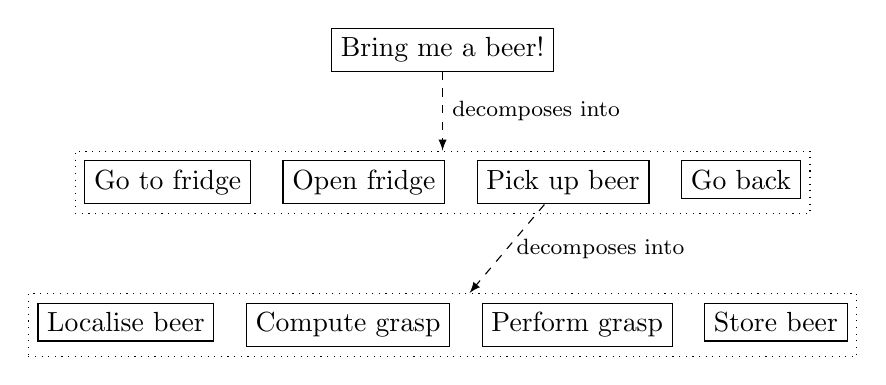
\begin{tikzpicture}[scale=0.3,>=latex,
                                ampersand replacement=\&, % needed when inside beamer frames
                                every node/.style={draw,solid},
                                every edge/.style={solid,ultra thick,<-,draw}]

                \node[draw=none] at (0,0) {}; % just to ensure a constant size for beamer
                \node[draw=none] at (0,-10) {}; % just to ensure a constant size for beamer

                \node<2-> (a1) {Bring me a beer!};

                \matrix<3->[dotted,below=of a1, matrix of nodes,column sep=4mm] (g1){
                        Go to fridge \& Open fridge \& Pick up beer \& Go back \\
                };

                \matrix<4->[dotted,below=of g1, matrix of nodes,column sep=4mm] (g2){
                    Localise beer \& Compute grasp \& Perform grasp \& Store beer \\
                };

                \draw<3->[dashed,->] (a1) -- (g1) node[draw=none,midway,right] {\footnotesize decomposes into};
                \draw<4->[dashed,->] (g1-1-3) -- (g2) node[draw=none,midway,right] {\footnotesize decomposes into};
            \end{tikzpicture}
    \end{center}
    }

    \only<5>{
        What \emph{primitive action} means is system-dependent: what an agent
        considers as primitive can be another agent’s plans.
    }

\end{frame}

\begin{frame}[fragile]{Task planning: actions}

    An action has \textbf{pre-conditions} and \textbf{post-conditions} (or \emph{effects}).

\begin{verbatim}
Action <action name>
{
    preconditions {...};
    effects{...};
    cost{<cost_function_name>};
    duration{<duration_function_name>};
}
\end{verbatim}

\pause

\begin{verbatim}
Action open_fridge
{
    preconditions {facing_fridge AND fridge_door.closed};
    effects {facing_fridge AND fridge_door.open};
}
\end{verbatim}

\end{frame}

\begin{frame}{Example: Shakey the robot}

    Shakey the robot (Stanford, 1968), using the \textbf{STRIPS} planner

    \begin{columns}
        \begin{column}{0.5\linewidth}
                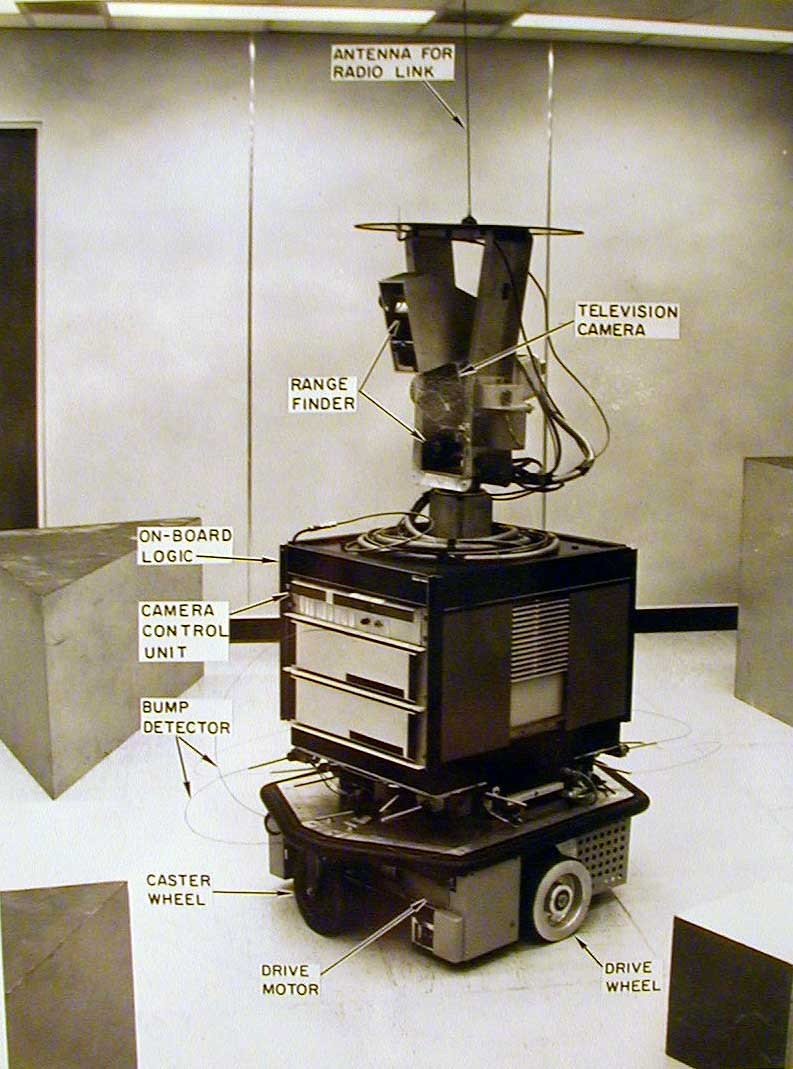
\includegraphics[width=0.8\linewidth]{shakey}
        \end{column}
        \begin{column}{0.5\linewidth}
                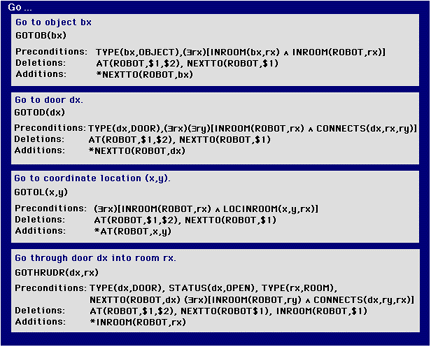
\includegraphics[width=\linewidth]{shakey-strips}
        \end{column}
    \end{columns}

\end{frame}

\videoframe[0.7]{figs/part7/clean-table.webm}

\begin{frame}{Task planning}

    \centering

        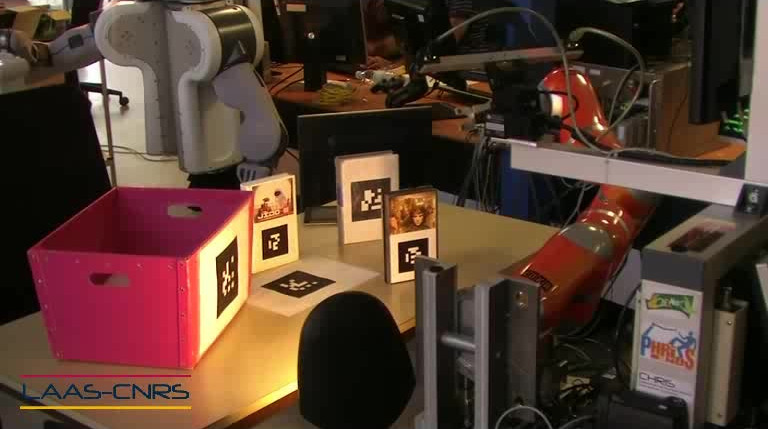
\includegraphics[width=0.7\linewidth]{clean-table}

    \resizebox{0.9\linewidth}{!}{%
        \begin{tikzpicture}[
                >=latex,
            robot/.style={fill=hriSec2Comp!50},
            every edge/.style={<-, draw, ultra thick},
            every node/.style={ draw, 
                        thick,  
                        circle, 
                        font=\sf,
                        align=center,
                        node distance=2cm,
                        fill=hriSec3CompDark!50, 
                        minimum size=3cm, 
                        inner sep=0.1cm}]

                    \node<2>[font=\rm\Huge, draw=none, fill=none, rotate=90] at (-3, 0) {Human\\actions};
            \node[font=\rm\Huge, draw=none, fill=none, rotate=90] at (-3, -4.5) {Robot\\actions};

            \coordinate (h1) at (0,0);

            \node<2> at (h1) (hh1) {\bf TAKE\\GREY\_TAPE\\TABLE};
            \node<2>[right=of hh1] (h2) {\bf PUT\\GREY\_TAPE\\BIN1 } edge (hh1);

            \node[robot, below=2.5 of h1] (r1) {\bf TAKE\\BLACK\_TAPE\\TABLE };
            \node[robot, right=of r1] (r2) {\bf PUT\\BLACK\_TAPE\\BIN2 } edge (r1);
            \node[robot, right=of r2] (r3) {\bf TAKE\\BOTTLE\\TABLE } edge (r2);
            \node[robot, right=of r3] (r4) {\bf PUTRV\\BOTTLE\\TABLE} edge (r3);
            \node[robot, right=of r4] (r5) {\bf TAKE\\BOOK\\TABLE } edge (r4);
            \node[robot, right=of r5] (r6) {\bf PUT\\BOOK\\BIN2 } edge (r5);

            \node<2> at (r5 |- h1) (h3) {\bf TAKE\\BOTTLE\\TABLE} edge (h2) edge (r4);
            \node<2>[right=of h3] (h4) {\bf PUT\\BOTTLE\\BIN1} edge (h3);

        \end{tikzpicture}
    }


\end{frame}


\begin{frame}[plain,label=cleantaskdiagram]{}
\centering
\resizebox{!}{0.9\paperheight}{%
\begin{tikzpicture}[
        >=latex,
        every edge/.style={draw, ultra thick, ->},
        every node/.style={align=center},
        robot/.style={fill=hriSec2Comp!50},
        plan/.style={draw,
                     thick,  
                     circle, 
                     font=\sf,
                     align=center,
                     fill=hriSec3CompDark!50, 
                     minimum size=1cm, 
                     inner sep=0.1cm}
        ]

        \coordinate<1> (figbottom) at (-0.5, -28.5);
        \coordinate<2-5> (figbottom) at (-0.5, -10.5);
        \node<2-5> at (0,5) {};
        \node<2-5> at ($(figbottom) + (0,-5)$) {};


        \fill[gray!10!white] (4.6,.5) rectangle (figbottom);

        \path (-0.5,0) edge (figbottom) node[sloped, above left, rotate=90] {\large\bf time};

        \node at (2,0) (percept) {\bf Perception};
            \node[below=0.5 of percept.south west, anchor=mid] {camera};
            \node[below=0.5 of percept.south east, anchor=mid] {3D model};

        \node[right=4 of percept, minimum width=2.5cm] (kb) {\bf Knowledge};
            \node[below=0.5 of kb.south west, anchor=mid east] (kbr) {robot};
            \node[below=0.5 of kb.south east, anchor=mid west] (kbh) {human};
            \draw[dotted] (kbr) to (figbottom -| kbr);
            \draw[dotted] (kbh) to (figbottom -| kbh);

        \fill[gray!10!white] (12,.5) rectangle (17,0 |- figbottom);
        \node[right=4.5 of kb] (plan) {\bf Plan};
            \node[below=0.5 of plan.south west, anchor=mid east] (probot) {robot};
            \node[below=0.5 of plan.south east, anchor=mid west] (phuman) {human};
            \draw[dotted] (probot) to (figbottom -| probot);
            \draw[dotted] (phuman) to (figbottom -| phuman);

        \node[right=5 of plan] (action) {\bf Actions};
            \node[below=0.5 of action.south west, anchor=mid east] (arobot) {robot};
            \node[below=0.5 of action.south east, anchor=west] (ahuman) {human\\(monitoring)};
            \draw[dotted] (arobot) to (figbottom -| arobot);
            \draw[dotted] (ahuman) to (figbottom -| ahuman);

        \draw[dashed] (-0.6,-1.2) --(24, -1.2);

        \node<1,2>[anchor=east] at (-0.5, -3) (t1) {\Large $t_1$};
        \node<1,2>[anchor=east, below=6 of t1] (t2) {\Large $t_2$};
        \node<3>[anchor=east] at (-0.5, -3) (t2) {\Large $t_2$};
        \node<1,3>[anchor=east, below=6 of t2] (t3) {\Large $t_3$};
        \node<4>[anchor=east] at (-0.5, -3) (t3) {\Large $t_3$};
        \node<1,4>[anchor=east, below=4 of t3] (t4) {\Large $t_4$};
        \node<5>[anchor=east] at (-0.5, -3) (t4) {\Large $t_4$};
        \node<1,5>[anchor=east, below=5 of t4] (t5) {\Large $t_5$};

        %%%%%%%%%%%%%%%%%%%%%%%%%%%%%%%%%%%%%%%%%%%%%%%%%%%%%%%%%%%%%%%%%%%%%%%%%%%%%%%%%%%%%%%%%%%%
        %%% PERCEPTIONS
        %%%%%%%%%%%%%%%%%%%%%%%%%%%%%%%%%%%%%%%%%%%%%%%%%%%%%%%%%%%%%%%%%%%%%%%%%%%%%%%%%%%%%%%%%%%%

        \node<1,2> at (t1 -| percept) (cam1) {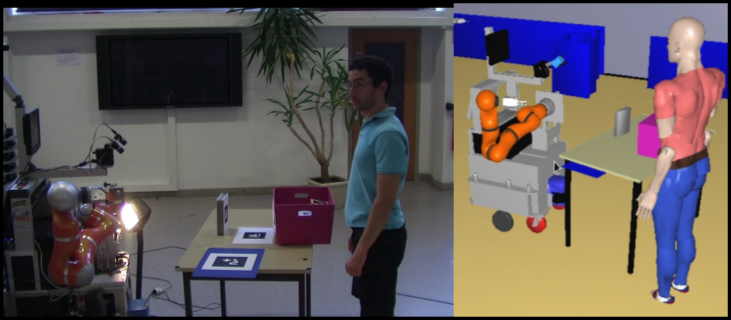
\includegraphics[height=2cm]{cleantable/manip_run_cam1.png}};
        \node<1,3> at (t2 -| percept) (cam2) {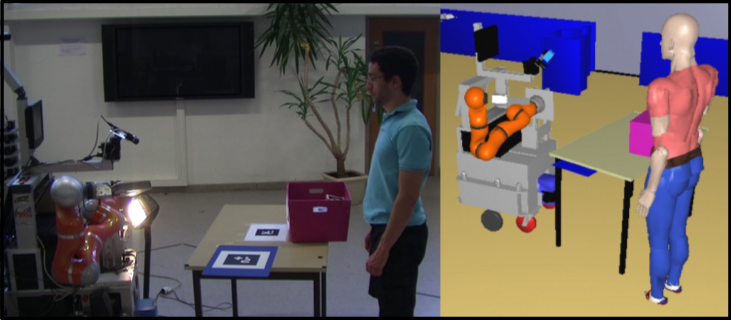
\includegraphics[height=2cm]{cleantable/manip_run_cam2.png}};
        \node<1,4> at (t3 -| percept) (cam3) {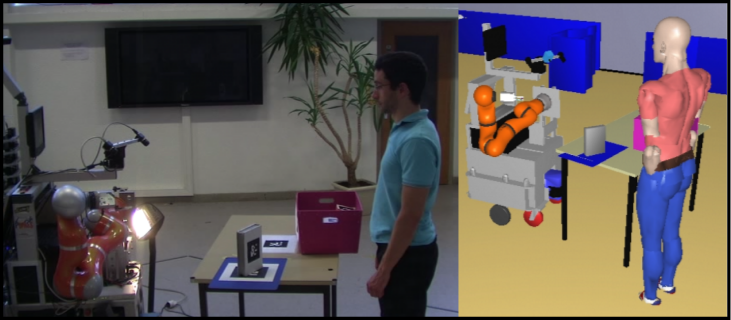
\includegraphics[height=2cm]{cleantable/manip_run_cam3.png}};
        \node<1,5> at (t4 -| percept) (cam4) {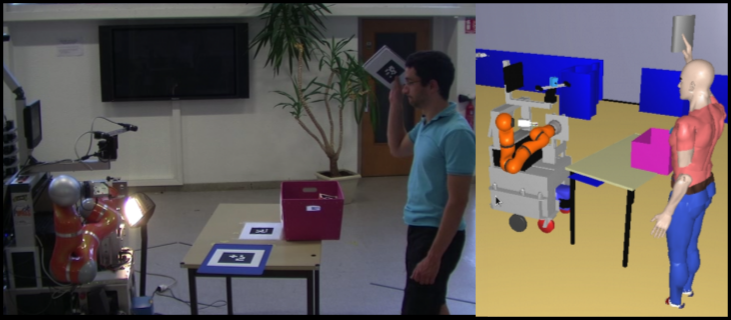
\includegraphics[height=2cm]{cleantable/manip_run_cam4.png}};
        \node<1,5> at (t5 -| percept) (cam5) {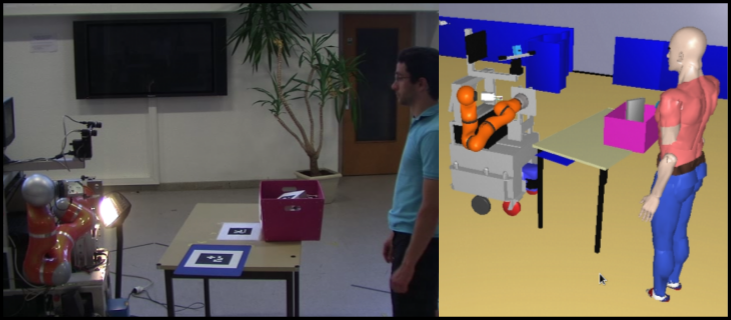
\includegraphics[height=2cm]{cleantable/manip_run_cam5.png}};

        %%%%%%%%%%%%%%%%%%%%%%%%%%%%%%%%%%%%%%%%%%%%%%%%%%%%%%%%%%%%%%%%%%%%%%%%%%%%%%%%%%%%%%%%%%%%
        %%% KNOWLEDGE
        %%%%%%%%%%%%%%%%%%%%%%%%%%%%%%%%%%%%%%%%%%%%%%%%%%%%%%%%%%%%%%%%%%%%%%%%%%%%%%%%%%%%%%%%%%%%

        \node<1,2>[fill=white,align=left] at (cam1 -| kbr) (kb1) {\stmt{TAPE isVisible true}\\
                                                        \stmt{TAPE isReachable true}\\
                                                        \stmt{TAPE isOn TABLE}\\
                                                        \stmt{BIN isVisible true}\\
                                                        \stmt{BIN isReachable false}};

        \node<1,2>[fill=white,align=left] at (cam1 -| kbh) {\stmt{TAPE isVisible true}\\
                                                        \stmt{TAPE isReachable false}\\
                                                        \stmt{TAPE isOn TABLE}\\
                                                        \stmt{BIN isVisible true}\\
                                                        \stmt{BIN isReachable true}};

        \node<1,3>[fill=white,align=left] at (cam2 -| kbr) (kb2) {\stmt{ROBOT hasInHand TAPE}};


        \node<1,4>[fill=white,align=left] at (cam3 -| kbr) {\stmt{TAPE isReachable true}\\
                                            \stmt{TAPE isVisible true} \\
                                            \stmt{TAPE isOn TABLE}};

        \node<1,4>[fill=white,align=left ] at (cam3 -| kbh) (kb3) {\stmt{TAPE isReachable true}\\
                                             \stmt{TAPE isVisible true}};

        \node<1,5>[fill=white,align=left] at (cam4 -| kbh) (kb4) {\stmt{HUMAN hasInHand TAPE}};

        \node<1,5>[fill=white,align=left] at (cam5 -| kbr)  {\stmt{TAPE isIn BIN}};
        \node<1,5>[fill=white,align=left] at (cam5 -| kbh) (kb5) {\stmt{TAPE isIn BIN}};

        %%%%%%%%%%%%%%%% %%%%%%%%%%%%%%%%%%%%%%%%%%%%%%%%%%%%%%%%%%%%%%%%%%%%%%%%%%%%%%%%%%%%%%%%%%%%
        %%% PLANS
        %%%%%%%%%%%%%%%%%%%%%%%%%%%%%%%%%%%%%%%%%%%%%%%%%%%%%%%%%%%%%%%%%%%%%%%%%%%%%%%%%%%%%%%%%%%%

        \node<1,2>[fill=gray!10!white,below=1 of plan] (incoming) {\bf \Large Incoming goal \\ \it Clean the table!};

        \node<1,2>[anchor=north, plan, robot] at (cam1.south -| probot) (pr1) {\bf TAKE\\TAPE\\TABLE};
        \node<1,3>[anchor=north, plan, robot] at (cam2.south -| probot)  (pr2) {\bf PUTRV\\TAPE\\TABLE} edge[<-] (pr1);
        \node<1,4>[anchor=north, plan] at (cam3.south -| phuman) (ph1) {\bf TAKE\\TAPE\\TABLE} edge[<-] (pr2);
        \node<1,5>[anchor=north, plan]  at (cam4.south -| phuman) (ph2) {\bf PUT\\TAPE\\BIN} edge[<-] (ph1);

        \node<1,5>[fill=gray!10!white,anchor=north] at (cam5.south -| plan) (done) {\bf \Large Goal completed};

        %%%%%%%%%%%%%%%%%%%%%%%%%%%%%%%%%%%%%%%%%%%%%%%%%%%%%%%%%%%%%%%%%%%%%%%%%%%%%%%%%%%%%%%%%%%%
        %%% ACTIONS
        %%%%%%%%%%%%%%%%%%%%%%%%%%%%%%%%%%%%%%%%%%%%%%%%%%%%%%%%%%%%%%%%%%%%%%%%%%%%%%%%%%%%%%%%%%%%

        \only<1,2>{
        \node[fill=white] at (pr1 -| arobot) (ep1) {\it evaluate pre-conditions};

        \node[below=0.1 of ep1] (mhp1) {%
            \begin{tikzpicture}
                \node[fill=white] (title) {\bf motion planning};
                \node[below=0.1 of title.south west, label=below:{\tt PICK\_GOTO}] (mapg) {
\includegraphics{cleantable/MHP_ARM_PICK_GOTO}};
                \node[fill=white,right=of mapg, label=below:{\tt TAKE\_TO\_FREE}] (mattf) {
\includegraphics{cleantable/MHP_ARM_TAKE_TO_FREE}} edge[<-] (mapg);
            \end{tikzpicture}
        };
        \node[fill=white,below=0.1 of mhp1] (me1) {\bf motion execution};
        \node[fill=white,below=0.1 of me1] (ae1) {\it assess post-conditions};
        }
        %%%%%%%%%%%%%%%%%%%%%%%%%%%%%%%%%%%%%%%%%%%%%%%%%%%%%%%%%%%%%%%%%%%%%%%%%%%%%%%%%%%%%%%%%%%%%
        \only<1,3>{
        \node[fill=white] at (pr2 -| arobot) (ep2) {\it evaluate pre-conditions};

        \node[below=0.1 of ep2] (mhp2) {%
            \begin{tikzpicture}
                \node[fill=white] (title) {\bf motion planning};
                \node[fill=white,below=0.1 of title, label=below:{\tt ESCAPE}] (maeo) {
\includegraphics{cleantable/MHP_ARM_ESCAPE_OBJECT}};
                \node[left=of maeo, label=below:{\tt PLACE\_FROM\_FREE}] (mapff) {
\includegraphics{cleantable/MHP_ARM_PLACE_FROM_FREE}} edge (maeo);
                \node[fill=white,right=of maeo, label=below:{\tt TO\_FREE}] (maf) {
\includegraphics{cleantable/MHP_ARM_FREE}} edge[<-] (maeo);
            \end{tikzpicture}
        };
        \node[fill=white,below=0.1 of mhp2] (me2) {\bf motion execution};
        \node[fill=white,below=0.1 of me2] (ae2) {\it assess post-conditions};
        }
        %%%%%%%%%%%%%%%%%%%%%%%%%%%%%%%%%%%%%%%%%%%%%%%%%%%%%%%%%%%%%%%%%%%%%%%%%%%%%%%%%%%%%%%%%%%%%

        \node<1,4>[anchor=north] at (ph1 -| ahuman) (wait1) {%
            \begin{tikzpicture}
                \node[fill=white] (title) {\it wait for pick\\ {\tt TAPE} \it from {\tt TABLE}};
                \node[below=0.1 of title] {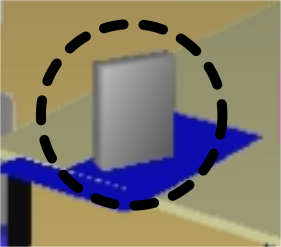
\includegraphics{cleantable/wait_for_pick}};
            \end{tikzpicture}
        };

        \node<1,5>[anchor=north] at (ph2 -| ahuman) (wait2) {%
            \begin{tikzpicture}
                \node[fill=white] (title) {\it wait for put\\ {\tt TAPE} \it into {\tt BIN}};
                \node[below=0.1 of title] {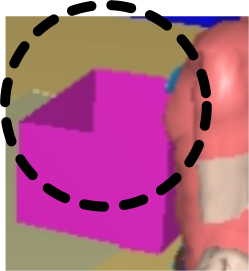
\includegraphics{cleantable/wait_for_throw}};
            \end{tikzpicture}
        };


        %%%%%%%%%%%%%%%%%%%%%%%%%%%%%%%%%%%%%%%%%%%%%%%%%%%%%%%%%%%%%%%%%%%%%%%%%%%%%%%%%%%%%%%%%%%%
        %%% FLOW
        %%%%%%%%%%%%%%%%%%%%%%%%%%%%%%%%%%%%%%%%%%%%%%%%%%%%%%%%%%%%%%%%%%%%%%%%%%%%%%%%%%%%%%%%%%%%
        \draw<1,2>[dotted, ->, in=45, out=180] (incoming.west) to (kb1);
        \draw<1,2>[dotted, ->, bend right] (kb1) to (pr1);
        \draw<1,2>[dotted, ->, bend left] (pr1) to (ep1);
        \draw<1,2>[dotted, ->, in=45, out=180] (ae1.west) to (kb2);
        \draw<1,3>[dotted, ->, bend right] (kb2) to (pr2);
        \draw<1,3>[dotted, ->, bend left] (pr2) to (ep2);
        \draw<1>[dotted, ->, in=45, out=180] (ae2.west) to (kb3);
        \draw<1,4>[dotted, ->, bend right] (kb3) to (ph1);
        \draw<1,4>[dotted, ->, bend left] (ph1) to (wait1);
        \draw<1>[dotted, ->, in=-20, out=180] (wait1.west) to (kb4.east);
        \draw<1,5>[dotted, ->, bend right] (kb4) to (ph2);
        \draw<1,5>[dotted, ->, bend left] (ph2) to (wait2);
        \draw<1,5>[dotted, ->, in=20, out=180] (wait2.west) to (kb5);
        \draw<1,5>[dotted, ->, bend left] (kb5.east) to (done.north);


 \end{tikzpicture}
 }
\end{frame}

\begin{frame}{Model/Plan/Act: strengths/weaknesses}

    {\bf Strengths}

    \begin{itemize}
        \item High-level goals are explicit
        \item Scale well with task complexity
        \item Easy to switch from one task to the other (planning domain is
            symbolic and explicit)

    \end{itemize}

    {\bf Weaknesses}

    \begin{itemize}
        \item Modeling and planning might be (very) computationally expensive
        \item Difficult to deal with unexpected events: not well suited for
            dynamic environments (often requires replanning)

    \end{itemize}

\end{frame}


%%%%%%%%%%%%%%%%%%%%%%%%%%%%%%%%%%%%%%%%%%%%%%%%%%%%

\begin{frame}{Finite state machines}

    \begin{center}
        \resizebox{\linewidth}{!}{
            \begin{tikzpicture}[>=latex,
                    every node/.style={thick,font=\bf},
                    every edge/.style={->,draw,thick,nodes={font=\scriptsize}}]

                \coordinate (origin) at (0,0);
                \node[minimum size=0.3cm, label={reset},fill,circle] at (origin) {};
                \node[draw,below right=of origin] (wait) {waiting};
                \node[draw,right=2 of wait] (blink) {blink red};
                \path (origin) edge[bend right]  (wait) 
                        (wait) edge node[above]{button press} (blink)
                               edge[loop below] node{no press} (wait);

                

                    \draw[<-,hriSec1Dark,ultra thick] (wait) -- ($(wait) + (80:1cm)$) node[draw=none,align=center,above,color=hriSec1Dark] {state};
                    \draw[<-,hriSec1Dark,ultra thick] (0.5,-1) -- +(250:1cm) node[draw=none,align=center,below,color=hriSec1Dark] {reset\\transition};
                    \draw[<-,hriSec1Dark,ultra thick] ($(wait.east) + (0.1,0)$) -- +(70:2cm) node[draw=none,align=center,above,color=hriSec1Dark] {transition};
                    \draw[<-,hriSec1Dark,ultra thick] ($(wait.east) + (1,0.5)$) -- +(50:1cm) node[draw=none,align=center,right,color=hriSec1Dark] {transition\\condition};

            \end{tikzpicture}
        }
    \end{center}
\end{frame}

\begin{frame}{Finite State Machine: wall avoidance example}
    \begin{center}
        \resizebox{0.7\linewidth}{!}{
            \begin{tikzpicture}[>=latex,
                every node/.style={thick,align=center,font=\bf},
                    every edge/.style={->,draw,ultra thick,nodes={align=center,font=\scriptsize}},
                    state/.style={draw,fill=hriSec2Comp!50,minimum width=2cm}
                    ]

                \path[use as bounding box] (-0.5, 3) rectangle (10, -6); % need to manually set the bb as the bezier curves used for the transition have control points far out

                \coordinate (origin) at (0,0);
                \node[minimum size=0.3cm, label={reset},fill,circle] at (origin) {};
                \node[state,below right=of origin] (move) {move\\forward};
                \node<2>[state] at ($(move) + (4,2)$) (right) {?};
                \node<3->[state] at ($(move) + (4,2)$) (right) {rotate\\right};
                \node<2>[state] at ($(move) + (4,-2)$) (left) {?};
                \node<3->[state] at ($(move) + (4,-2)$) (left) {rotate\\left};

                \path (origin) edge[bend right]  (move);
                 \path<2> (move.east) edge[out=0,in=180] (right)
                                      edge[out=0,in=180] (left)
                                      edge[out=0,in=-90,looseness=3] (move.south);
                 \path<3-> (move.east) edge[out=0,in=180] node[right]{left sensor\\detect wall} (right)
                                       edge[out=0,in=180] node[right]{right sensor\\detect wall} (left)
                                       edge[out=0,in=-90,looseness=4] node[below]{no wall} (move.south);

                 \path<4> (right.east) edge[out=0,in=-90,looseness=4] node[right]{?} (right.south)
                                       edge[out=30,in=90,looseness=2] node[above]{?} (move.north)
                           (left.east) edge[out=0,in=90,looseness=4] node[right]{?} (left.north)
                                       edge[out=-30,in=-90,looseness=2] node[below]{?} (move.south);
                 \path<5-> (right.east) edge[out=0,in=-90,looseness=4] node[right]{$|angle| < \pi/2$} (right.south)
                                       edge[out=30,in=90,looseness=2] node[above]{$|angle| \geq \pi/2$} (move.north)
                           (left.east) edge[out=0,in=90,looseness=4] node[right]{$|angle| < \pi/2$} (left.north)
                                       edge[out=-30,in=-90,looseness=2] node[below]{$|angle| \geq \pi/2$} (move.south);

            \end{tikzpicture}
        }
    \end{center}
    \source{https://www.clear.rice.edu/engi128/Handouts/Lec17-Robotics.pdf}{example borrowed from Rice University ENGI128}
\end{frame}

\imageframe{fsm-pr2-charging}
\videoframe[0.56]{figs/part7/cowriter.mp4}
\imageframe[scale=0.8]{cowriter-fsm}

\begin{frame}{FSM with ROS: the SMACH package}
    \href{http://wiki.ros.org/smach}{\textbf{SMACH}} is a ROS-independent (but very weill integrated with ROS!) Python library to build state machines

    \begin{itemize}
        \item support for hierarchical (\ie nested) state machines
        \item provides support for concurrency as well
    \end{itemize}

    \begin{center}
        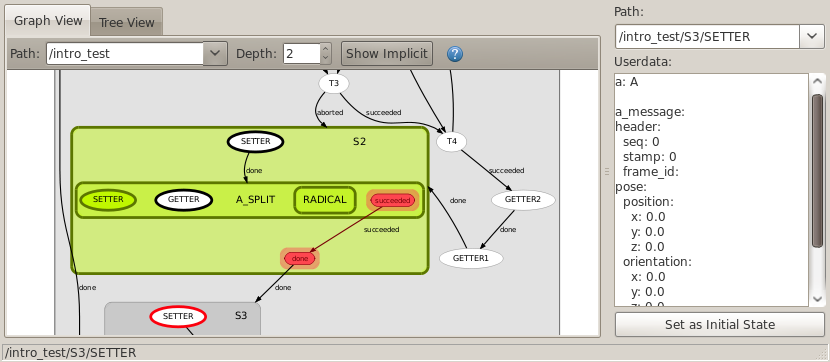
\includegraphics[width=0.8\linewidth]{smach}
    \end{center}
\end{frame}


\begin{frame}{Relation to behavioural/deliberative paradigms}

    Finite State Machines are \textbf{not a control paradigm} per-se.

    Instead, they are a mathematical formalism to describe states and transitions.

    States themselves might be behavioural components, deliberative components,
    or \textbf{nested state machines}.

\end{frame}

\begin{frame}{Finite State Machine: strengths/weaknesses}

    {\bf Strengths}

    \begin{itemize}
        \item Behaviour formally provable
        \item Easier to debug: control flow is explicit
    \end{itemize}

    {\bf Weaknesses}

    \begin{itemize}
        \item Less modular than behavioural approaches
        \item Difficult to deal with unexpected events: not well suited for dynamic environments
    \end{itemize}


\end{frame}


%%%%%%%%%%%%%%%%%%%%%%%%%%%%%%%%%%%%%%%%%%%%%%%%%%%%
%%%%%%%%%%%%%%%%%%%%%%%%%%%%%%%%%%%%%%%%%%%%%%%%%%%%%%%%%%%%%%%

\section{Control Architectures}

\begin{frame}<1-2>[label=ctrlstrategies]{Control strategies so far}

    {\bf Behavioural} or reactive

    \begin{itemize}
        \item \emph{bottom-up} approach
        \item lots of independent modules executing concurrently,
            monitoring sensor values, triggering actions and possibly inhibiting each-others
        \item hard to organize into complex behaviours; gets messy quickly
    \end{itemize}

    \pause

    {\bf Hierarchical}: classic model/plan/act

    \begin{itemize}
        \item \emph{top-down} approach
        \item starts with high-level goals, decompose into sub-tasks
        \item not very agile
    \end{itemize}

    \pause

    {\bf Hybrid approaches?}

    \begin{itemize}
        \item Deliberative at high level, reactive at low level
    \end{itemize}

\end{frame}

\begin{frame}{Subsumption architecture}

        \begin{center}
            \resizebox{0.9\linewidth}{!}{
                \begin{tikzpicture}[>=latex,
                                    every node/.style={draw,minimum width=2cm}]
                    \node at (0,0) (l0) {level 0};
                    \node[above=1 of l0] (l1) {level 1};
                    \node[above=1 of l1] (l2) {level 2};
                    \node[above=1 of l2] (l3) {level 3};
                    \coordinate[above=1 of l3] (l4);

                    \node[left=2 of l0,draw=none] (sensors) {\bf Sensors};

                    \draw[->] (sensors) -- (l0);

                    \coordinate[left=1 of l0] (s0);
                    \draw[->] (s0) |- (l1);
                    \draw[->] (s0) |- (l2);
                    \draw[->] (s0) |- (l3);
                    \draw[dashed] (s0 |- l3) |- +(0,1);

                    \coordinate[right=3 of l0] (s1);
                    \coordinate[right=2 of l1] (s2);
                    \coordinate[right=1 of l2] (s3);


                    \node[circle,ultra thick,fill=hriSec2Dark,minimum size=5mm] at (s1) (ss1) {\bf S};
                    \draw[->] (l0) -- (ss1);
                    \draw[->] (l1) -| (ss1);
                    \node[circle,ultra thick,fill=hriSec2Dark,minimum size=5mm] at (s2) (ss2) {\bf S};
                    \draw[->] (l2) -| (ss2);
                    \node[circle,ultra thick,fill=hriSec2Dark,minimum size=5mm] at (s3) (ss3) {\bf S};
                    \draw[->] (l3) -| (ss3);

                    \draw[dashed] (l3 -| s3) |- +(0,1);

                    \node[right=5 of l0,draw=none] (act) {\bf Actuators};

                    \draw[->] (ss1) -- (act);


                \end{tikzpicture}
            }
        \end{center}


        \source{http://dspace.mit.edu/bitstream/handle/1721.1/6432/AIM-864.pdf}{Brooks, A robust layered control system for a mobile robot, 1986}
\end{frame}

\imageframe[caption={Level 0: obstacle avoidance}]{subsumption-arch-1}
\imageframe[caption={Level 1: wander around aimlessly}]{subsumption-arch-2}
\imageframe[caption={Level 2: exploratory behaviour}]{subsumption-arch-3}

\begin{frame}{Example: the MIT Genghis robot}


    \begin{columns}
        \begin{column}{0.5\linewidth}

            MIT Genghis: Rodney Brooks in 1989

            Really simple hardware


            \begin{itemize}

                \item 6 legs, 2 motors per leg
                    \begin{itemize}
                        \item motor for forward/back, motor for up/down
                    \end{itemize}
                \item 2 bump sensors (feelers)
                \item 2 ground detection sensors (switches)
                \item 6 heat sensors (but they weren’t used for walking)
            \end{itemize}
        \end{column}
        \begin{column}{0.5\linewidth}

            \begin{center}
                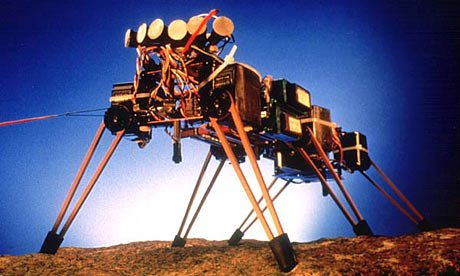
\includegraphics[width=\linewidth]{genghis}
            \end{center}
        \end{column}
    \end{columns}
\end{frame}

\videoframe[0.7]{figs/part7/genghis-short2.mov}

\imageframe[caption={In total, 57 FSMs}]{genghis-subsumption}

\againframe<3>{ctrlstrategies}

\begin{frame}{Levels of control}
    Control problems are usually split into three levels:

    \begin{itemize}
        \item<1-> \textbf{Low-level control}
            \begin{itemize}
                \item Example: where to place a leg as robot takes its next step
                \item Generally, continuous-valued problems
                \item Short time scale (under a second); high frequency loop
            \end{itemize}
        \item<2-> \textbf{Intermediate level control}
            \begin{itemize}
                \item Navigating to a destination, or picking up an object
                \item Continuous or discrete valued problems
                \item Time scale of a few seconds
            \end{itemize}
        \item<3-> \textbf{High level control}
            \begin{itemize}
                \item What is the plan for moving these boxes out of the room?
                \item Discrete problems, long time scale (minutes)
            \end{itemize}
    \end{itemize}

    \source{https://www.cs.cmu.edu/afs/cs/academic/class/15494-s11/lectures/architectures.pdf}{CMU lecture on Cognitive Robotics}
\end{frame}

\begin{frame}{Layered Architectures}
    \begin{center}
        %\resizebox{\linewidth}{!}{
            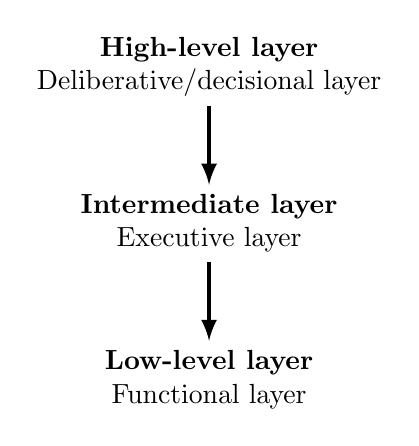
\begin{tikzpicture}[>=latex,every node/.style={minimum width=4cm,align=center}]
                
                \node (low) {\bf Low-level layer\\Functional layer};
                \node[above=of low] (mid) {\bf Intermediate layer\\Executive layer} edge[ultra thick,->] (low);
                \node[above=of mid] (hig) {\bf High-level layer\\Deliberative/decisional layer} edge[ultra thick,->] (mid);

            \end{tikzpicture}
        %}
    \end{center}

    Each layer has different time constraints (from real-time to possibly `slow'); they typically use different control paradigms
\end{frame}


\begin{frame}{Deliberative architecture for interaction}

    One example: the LAAS deliberative architecture for interaction

    \begin{center}
        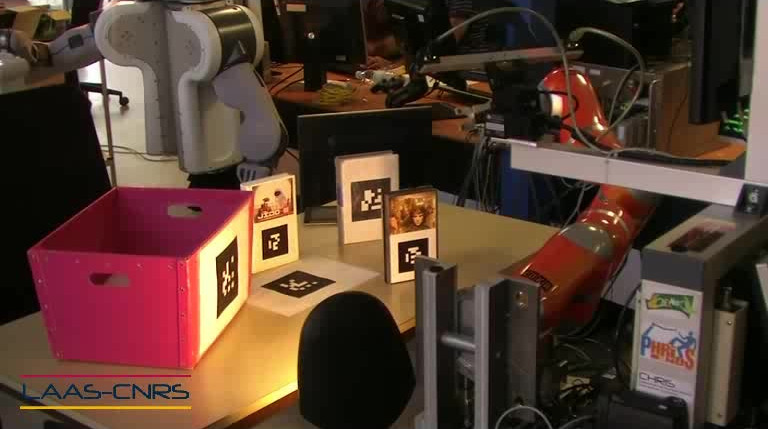
\includegraphics[width=0.8\linewidth]{clean-table}
    \end{center}
\end{frame}

\againframe<1>[plain]{cleantaskdiagram}

\begin{frame}<1-6>[label=laasarch]{Deliberative architecture for interaction}

\resizebox{\paperwidth}{!}{%

\tikzset{subpart/.style={draw, font=\scriptsize, fill opacity=0.5, text opacity=1, fill=white!50}}
\begin{tikzpicture}[
    >=latex,
    every edge/.style={draw, very thick},
    skill/.style={draw, rounded corners, align=center, inner sep=5pt, fill=black!20},
    stmt/.style={align=center, font=\bf},
    label/.style={midway, align=center, font=\scriptsize, fill=white}]

  %%% LOWLEVEL
 \uncover<+->{
  \node [skill] (lowlevel) {%
      \begin{tikzpicture}
        \node at (0,0) (sensori) {Sensorimotor layer};
        %\node [subpart, below=0.2 of sensori.south west, anchor=north west, align=left] (perception) {{\bf Perception} \\ 2D markers, RGB-D, motion capture};
        %\node [subpart, align=right, right=0.2 of perception] {{\bf Actuation} \\ Head's pan-tilt unit, grippers, arms, wheels};
      \end{tikzpicture}
  };
}

 \uncover<+->{
  %%% SITUATION ASSESSMENT
  \node [skill, above=2 of lowlevel, fill=hriSec3!50] (spark) {%
      \begin{tikzpicture}
          \node at (0,0) (geom) {{\bf Situation Assessment} -- geometric \& temporal reasoning};
        \node [subpart, below=0.2 of geom.south west, anchor=north west] (world-update) {Sensors fusion};
        \node [subpart, right=0.2 of world-update] (geom-model) {Geometric model of the environment};
        \node [subpart, right=0.2 of geom-model] (fact-prod) {Symbolic facts production};
      \end{tikzpicture}
    };

    \path (lowlevel) edge [->] (spark);
  }


 \uncover<+->{
  %%% KB
    \node [skill, above=3 of spark.west, fill=hriSec2Dark!50] (oro) {{\bf Memory} knowledge base(s)\\ \footnotesize typically a symbolic blackboard};
    \path (spark.100) edge [->, bend right] node[label] (symfact) {symbolic \\ facts} (oro);
    }

 \uncover<+->{
   %%% SUPERVISION
  \node [skill, above=6 of spark,fill=hriSec1Comp!50] (shary) {%
      \begin{tikzpicture}
          \node at (0,0) (exec) {\bf Supervision (Execution Controller)};
        \node [subpart, below=0.2 of exec.south west, anchor=north west] (plans) {Goal \& Plans \\ management};
        \node [subpart, right=0.2 of plans] (sit-asses) {Situation assessment \\ and context management};
        \node [subpart, right=0.2 of sit-asses] {Action instantiation, \\ execution and monitoring};
      \end{tikzpicture}
    };
  \path (shary) edge [<->, bend left] node[label] (evts) {events, \\ world model and \\ agents beliefs} (oro);
  \path (shary) edge [<->, bend left] node[label] {action monitoring \\ and management of \\ position hypotheses} (spark);
  \path (lowlevel.east) edge [<-, bend right=80, looseness=1.5] node[label] {atomic\\actions} (shary.east);
 }
  

 \uncover<+->{
  %%% HATP
    \node [skill, left=5 of shary.south west,fill=hriSec1!50] (hatp) {{\bf Task planner}\\ \footnotesize ideally human-aware};

  %%% MHP
    \node [skill, below=3 of shary.east,fill=hriSec3CompDark!50] (mhp) {Motion and manipulation \\ planning};
  \path (shary.340) edge [<->, bend left] node[label] {motion plan \\ requests} (mhp);
  \path (shary.west) edge [<->, bend right] node[label] {shared \\ plans} (hatp);
  \path (hatp) edge [<->, bend right] node[label] (domain) {world model and \\ agents beliefs} (oro.170);
  \path (spark.5) edge [->, bend right] node[label] {environment\\model} (mhp);

 }

 \uncover<+->{
  %%% DIALOGS
    \node [skill, left=3 of spark,fill=hriSec3Dark!50] (dialogs) {{\bf Multi-modal communication}\\NLP, back-channel,...};
    \path (dialogs) edge [<->, bend left] node[label] (nlp) {natural language \\ grounding} (oro.190);

  }
 

  %%% Separation between deliberative layer and sensori-motor layer
  \coordinate (mid) at ($(lowlevel)!0.5!(spark)$);
  \draw[dotted, thick] (dialogs.west |- mid) -- (mhp.east |- mid);

  \only<7>{
      \fill[fill opacity=.7,white] (current bounding box.north west) rectangle (current bounding box.south east);
      \node[stmt] at (symfact) {isOn(bottle, table)\\lookAt(human1, bottle)};
      \node[stmt] at (nlp) {lookAt(human1, ?obj)\\desires(human1, PickUp, bottle)};
      \node[stmt] at (domain) {isAvailable(?gripper)\\ $\wedge$ isA(?gripper, Gripper)\\isOn(bottle, ?obj)};
      \node[stmt] at (evts) {isA(action23425, PickUp)\\ $\wedge$ currentlyPerforming(action23425)};
  }
\end{tikzpicture}
}
\end{frame}

\begin{frame}{}

    How do modules actually communicate with each other?

\end{frame}

\againframe<7>{laasarch}

%%%%%%%%%%%%%%%%%%%%%%%%%%%%%%%%%%%%%%%%%%%%%%%%%%%%%%%%%%%%%%%
%%%%%%%%%%%%%%%%%%%%%%%%%%%%%%%%%%%%%%%%%%%%%%%%%%%%%%%%%%%%%%%

%\section{Cognitive Architectures}
%
%\begin{frame}{Investigating robot cognition}
%    \begin{center}
%        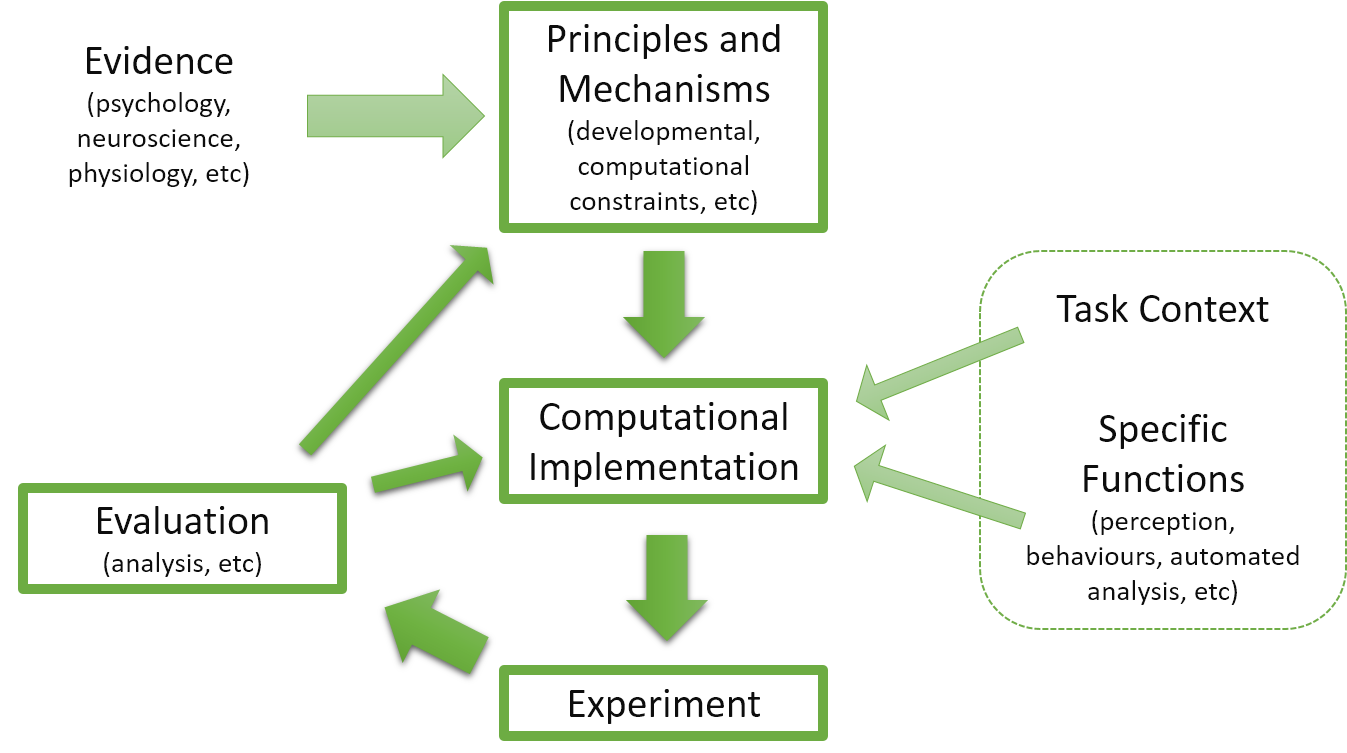
\includegraphics[width=0.8\linewidth]{cogarch}
%    \end{center}
%\end{frame}
%
%\begin{frame}{Architectures to model human cognition}
%
%\resizebox{!}{0.7\paperheight}{%
%\tikzset{subpart/.style={draw, font=\scriptsize, fill opacity=0.5, text opacity=1, fill=white!50}}
%\begin{tikzpicture}[
%    >=latex,
%    node distance=1.5,
%    every edge/.style={draw, very thick},
%    skill/.style={draw, rounded corners, align=center, inner sep=5pt, fill=black!20},
%    stmt/.style={align=center, font=\bf},
%    label/.style={midway, align=center, font=\scriptsize, fill=white}]
%
%    \node at (0,0)[skill, fill=hriSec2!50] (a1) {Shared Plan Elaboration};
%
%    \node [skill, fill=hriSec2!50,above=of a1] (a2) {Intention Prediction};
%    \node [skill, fill=hriSec2!50,left=of a1] (a3) {Mental State Management};
%    \node [skill, fill=hriSec2!50,right=of a1] (a4) {Communication for\\Joint Action};
%    \node [skill, fill=hriSec2!50,below=of a1] (a5) {Shared Plan Achievement};
%    \node [skill, fill=hriSec2!50,left=of a5] (a6) {Situation Assessment};
%
%
%    \node [skill, fill=hriSec3!50,below left=of a5,anchor=north] (a7) {Action Achievement};
%    \node [skill, fill=hriSec3!50,below right=of a5,anchor=north] (a8) {Human Action Monitoring};
%  
%    \node[below=3.7 of a5] (a14) {Human-aware geometric and task planners, real-time controllers, sensors...};
%
%  \coordinate[below=3 of a6] (a9);
%
%  \node[rotate=90,left=0.7 of a3.west] (distal) {\bf\large DISTAL};
%  \node[rotate=90] at (distal |- a7.south) {\bf\large PROXIMAL};
%  \node[rotate=90] at (distal |- a14) {\bf\large MOTOR};
%
%  \coordinate (a11) at (a9 -| distal.north);
%  \coordinate (a12) at (a9 -| a4.east);
%  \draw[dotted, thick] (a11) -- (a12);
%
%
%  \coordinate (a13) at ($(a5)!0.5!(a7)$);
%  \draw[dotted, thick] (a13 -| distal.north) -- (a13 -| a4.east);
%
%
%  %%% Relations between components
%  \path (a2) edge [->] node[label] {goal to execute} (a1);
%  \path (a1) edge [->] node[label] {plan} (a5);
%  \path (a2) edge [<-] node[label] {goal (order)} (a4);
%
%  \path (a3) edge [<->, bend left=40, looseness=1.2] node[label,pos=0.1] {mental state information} (a4);
%  \path (a3) edge [<->] (a2);
%  \path (a3) edge [<->] (a1);
%  \path (a3) edge [<->] (a5);
%
%  \path (a6) edge [->] node[label] {conceptual\\world state} (a3);
%
%  \path (a5) edge [<->] node[label] {coordination} (a4);
%
%  \path (a5) edge [<->] node[label,right=0.5] {anchoring of actions} (a7);
%  \path (a5) edge [<->] (a8);
%
%  \path (a9) edge [->] node[label] {sensors} (a6);
%
%  \coordinate (a10) at (a9 -| a7);
%  \path (a10) edge [<->] node[label] {planning and control} (a7);
%
%  \coordinate (a10) at (a9 -| a8);
%  \path (a10) edge [<->] node[label] {sensors} (a8);
%
%  \path (a7) edge [<->] node[label] {coordination} (a8);
% 
%\end{tikzpicture}
%}
%
%\source{}{Sandra Devin}
%\end{frame}
%
%%%%%%%%%%%%%%%%%%%%%%%%%%%%%%%%%%%%%%%%%%%%%%%%%%%%%
%%%%%%%%%%%%%%%%%%%%%%%%%%%%%%%%%%%%%%%%%%%%%%%%%%%%

\section{Middlewares}

\begin{frame}{Robotic middlewares}
 The core role of a \textbf{middleware} is to \textbf{provide a set of abstractions to ease the development of robotic software components}.

    \begin{itemize}
        \item<+-> It \textbf{abstracts away the hardware platform} (uniform driver interfaces)
        \item<+-> It abstracts away where computations are physically performed (by providing
            \textbf{distributed computation/network transparency})

        \item<+-> It supports \textbf{modularity}/\textbf{reusability} (\textbf{standard interfaces}: modules which
            implement these interfaces can be easily swapped)
        \item<+-> It help with debugging (by providing \textbf{introspection} mechanisms)

    \end{itemize}

\end{frame}

\begin{frame}{Middlewares in a broader sense}
    \begin{center}
        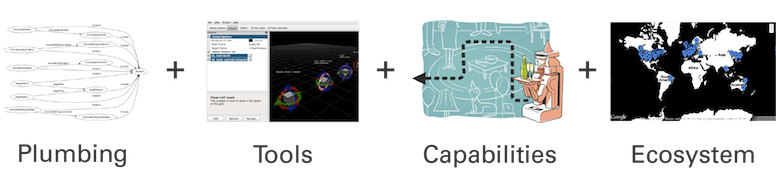
\includegraphics[width=\linewidth]{ros_equation}
    \end{center}
\end{frame}

\begin{frame}{Existing middlewares}
    \begin{itemize}
        \item OROCOS (Europe)
        \item YARP (Europe)
        \item OpenRTM (Korea)
        \item \textbf<2>{ROS} -- Robot Operating System (originally US)
        \item OpenRAVE (US)
    \end{itemize}
\end{frame}

\begin{frame}{ROS}

    \begin{center}
        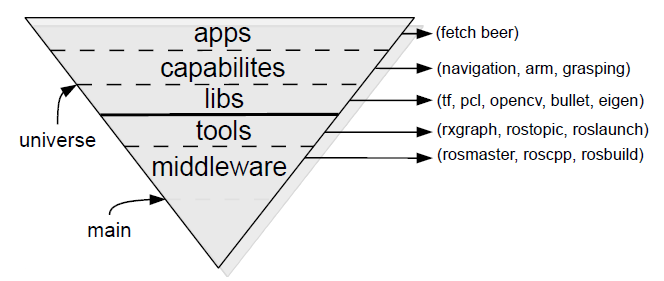
\includegraphics[width=\linewidth]{ros_structure}
    \end{center}
\end{frame}

\begin{frame}{Talking Nodes}

\begin{center}
\begin{tikzpicture}[
                    >=latex,
                    every edge/.style={->, draw, very thick},
                    service/.style={->, draw, very thick,dashed},
                    rosnode/.style={draw, font=\sf, node distance=0.5, rounded
                    corners, align=center, inner sep=5pt,fill=hriSec2Dark!50},
                    topic/.style={font=\tt, node distance=0.5, align=center, inner sep=5pt},
                    pic/.style={fill=none,draw=none}
                ]

    \path[use as bounding box] (-6,1) rectangle (6,-5);
    \node [rosnode] at (0,0) (node1) {node 1};
    \node [rosnode] at (4,-2) (node2) {node 2};
    \node [rosnode] at (-5,-4) (node3) {node 3};

    \uncover<2-> {
        \node [topic] at (1,-2) (topic1) {/topic1};
        \node [topic] at (-1,-3) (topic2) {/topic2};
        \node [topic] at (-4,-2) (topic3) {/topic3};
        \path (node1) edge[bend left] node[label,right] {\only<2-3>{publishes}} (topic1);
        \path (node1) edge[bend right] node[label,left] {\only<2-3>{publishes}} (topic2);
        \path (node3) edge[bend left] node[label,left] {\only<2-3>{publishes}} (topic3);
    }
    \uncover<3-> {
        \path (topic1) edge[bend right] node[label,below left] {\only<3>{subscribes}} (node2);
        \path (topic2) edge[bend left] node[label,below] {\only<3>{subscribes}} (node3);
        \path (topic2) edge[bend right] (node2);
    }
    \only<4-5> {
        \path[->, dashed] ([yshift=2pt]node1.east) edge[bend left] node[label,above right] {service (RPC)} ([xshift=2pt]node2.north) ;
    }
    \only<5> {
        \path[->, dashed] ([xshift=-2pt]node2.north) edge[bend right] ([yshift=-2pt]node1.east);

    }

    \uncover<6-> {
        \path[->, dashed] ([yshift=2pt]node1.east) edge[bend left] node[label,above right] {\only<6,7>{action goal}} ([xshift=2pt]node2.north) ;
    }
    \uncover<7-> {
        \path[->, dashed] ([xshift=-2pt]node2.north) edge[bend right] node[label,below left] {\only<7>{result}} ([yshift=-2pt]node1.east);

    }

    \only<8> {
        \node [rosnode,fill=hriSec3!50] at (-5,0) (roscore) {roscore};
        \path[dashed] (node1) edge[<->,very thin, bend right] node[label,above] {\tiny XML-RPC} (roscore);
        \path[dashed] (node2) edge[<->,very thin, bend right] node[label,above] {\tiny XML-RPC} (roscore);
        \path[dashed] (node3) edge[<->,very thin, bend left] node[label,above right] {\tiny XML-RPC} (roscore);

    }

\end{tikzpicture}
\only<5>{Services: \bf synchronous}
\only<7>{Actions: \bf asynchronous}
\only<8>{\tt ROS\_MASTER\_URI=http://<host>:<port>}
\end{center}

\end{frame}


\begin{frame}{ROS}
    \begin{itemize}
        \item<1-> A fairly simple peer-to-peer message passing system designed with robotics in
            mind
        \item<2-> An API to this system (in several languages -- C++ and Python are
            1st tier)
        \item<3-> A set of standard message types that facilitate interoperability between modules
        \item<4> \bf{A middleware?}
        \item<5-> A set of conventions to write and package robotic softwares
        \item<6-> Deep integration of a few key open-source libraries (OpenCV, PCL, tf)
        \item<7-> A set of tools to run and monitor the nodes
        \item<8-> Engagement of a large academic community, leading to a library of thousands of nodes
    \end{itemize}
\end{frame}

\begin{frame}{ROS Ecosystem}
    \centering
    \resizebox{0.9\textwidth}{!}{%
        \vspace*{4cm}
        \begin{tikzpicture}

            \path[small mindmap,
                  level 1 concept/.append style={sibling angle=360/5}, 
                  level 2 concept/.append style={sibling angle=60}, 
                  concept color=hriWarmGreyLight,text=hriWarmGreyDark]

            node[concept] {\bf ROS}
            [clockwise from=-180]
            child[concept color=hriSec1Dark,text=white] { node[concept]{Middleware} 
                [clockwise from=-120]
                child[concept color=hriSec1CompDark,text=white] { node[concept]{Standard Interfaces} }
                child[concept color=hriSec3CompDark,text=white] { node[concept]{Nodes Management} }
                child[concept color=hriSec2Dark,text=white] { node[concept]{IPC} }
            }
            child[concept color=hriSec3Comp,text=white] { node[concept] {Standards and Conventions} }
            child[concept color=hriSec2CompDark,text=white] { node[concept]{Community}
                [clockwise from=90]
                child[concept color=hriSec2Comp,text=white] { node[concept]{Software engineering infrastructure} }
                child[concept color=hriSec1,text=white] { node[concept] {REPs} }
                child[concept color=hriSec3,text=white] { node[concept] {ROSCon} }
            }
            child[concept color=hriSec3Dark,text=white] { node[concept] {Large software library} 
                [clockwise from=0]
                child[concept color=hriSec2Dark,text=white] { node[concept] {Satellite libraries} }
            }
            child[concept color=hriSec3CompDark,text=white] { node[concept] {Tooling} };
        \end{tikzpicture}
    }
\end{frame}

\begin{frame}{Example: a simple image processing pipeline}

\begin{center}
\begin{tikzpicture}[
                    >=latex,
                    every edge/.style={->, draw, very thick},
                    service/.style={->, draw, very thick,dashed},
                    rosnode/.style={draw, font=\sf, node distance=0.5, rounded
                    corners, align=center, inner sep=5pt,fill=hriSec2Dark!50},
                    topic/.style={font=\tt, node distance=0.5, align=center, inner sep=5pt},
                    pic/.style={fill=none,draw=none}
                ]

    \node [rosnode] at (-4,0) (node1) {image acquisition};
    \node [rosnode] at (0,-2) (node2) {image processor};
    \node [rosnode] at (4,-4) (node3) {next processing};

        \node [topic] at (-4,-1.5) (topic3) {/image};
        \node [topic] at (-1,-3.5) (topic1) {/processed\_image};
        \path (node1) edge[bend right] (node2);
        \path (node2) edge[bend right] (node3);


\end{tikzpicture}
\end{center}

\end{frame}

\begin{frame}[containsverbatim]{}

\begin{pythoncode}
import sys, cv2, rospy
from sensor_msgs.msg import Image
from cv_bridge import CvBridge

def on_image(image):
    cv_image = bridge.imgmsg_to_cv2(image, "bgr8")
    (rows,cols,channels) = cv_image.shape
    cv2.circle(cv_image, (cols/2,rows/2), 50,(0,0,255), -1)
    cv2.imshow("Image window", cv_image)
    cv2.waitKey(3)
    image_pub.publish(bridge.cv2_to_imgmsg(cv_image, "bgr8"))

rospy.init_node('image_processor')
bridge = CvBridge()
image_sub = rospy.Subscriber("image",Image, on_image)
image_pub = rospy.Publisher("processed_image",Image)

while not rospy.is_shutdown():
    rospy.spin()
\end{pythoncode}

\end{frame}

\begin{frame}[containsverbatim]{}

\begin{shcode}
$ roslaunch gscam v4l.launch
$ python image_processor.py image:=/v4l/camera/image_raw
$ rosrun image_view image_view image:=/processed_image
\end{shcode}

\end{frame}



\begin{frame}{}
    \begin{center}
        \Large
        That's all, folks!\\[2em]
        \normalsize
        Questions:\\
        Portland Square A216 or \url{severin.lemaignan@plymouth.ac.uk} \\[1em]

        Slides:\\ \href{https://github.com/severin-lemaignan/module-mobile-and-humanoid-robots}{\small github.com/severin-lemaignan/module-mobile-and-humanoid-robots}

    \end{center}
\end{frame}



\end{document}
